\section{Dettagli Implementativi}

\subsection{Dialoghiamo}
\begin{frame}{Dialoghiamo}
  Il processo che prende il nome di "Dialoghiamo" è una sorta di \emph{hub} volto alla comunicazione.

  La sezione "la vostra voce" nello specifico funge da bacino in cui pensieri e idee nascono e si alimentano

  per poi eventualmente assumere una forma più \emph{ufficiale} nella sezione "Decidiamo"
\end{frame}
\subsection{Decidiamo}
\begin{frame}{Decidiamo - Le Fasi}
  Il processo decidiamo è suddiviso in fasi

  \pause
  Le fasi vengono riattivate periodicamente, alla fine di ogni ciclo i cittadini possono avanzare nuove proposte.


  \begin{center}
    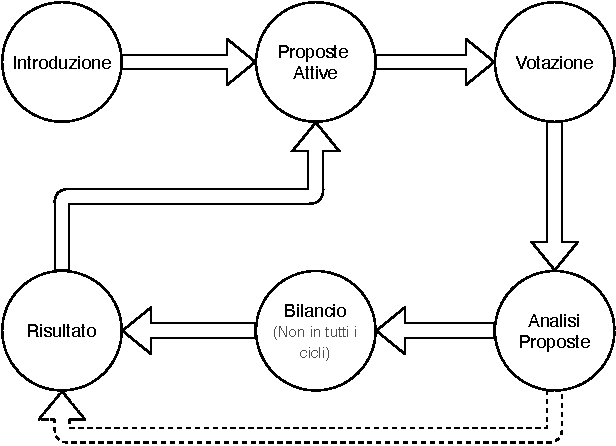
\includegraphics[width=0.7\textwidth]{Fasi}
  \end{center}
\end{frame}
\begin{frame}

  \begin{table}
    \renewcommand\arraystretch{1.4}\arrayrulecolor{LightSteelBlue3}

    \begin{tabular}{@{\,}r <{\hskip 2pt} !{\foo} >{\raggedright\arraybackslash}p{5cm}}

      \addlinespace[1.5ex]
      Introduzione     & \small{Fase inziale}                                                      \\
      Proposte Attive  & \small{I cittadini possono avanzare proposte}                             \\
      Votazione        & \small{I cittadini votano le proposte  }                                  \\
      Analisi Proposte & \small{L'azienda considera le proposte}                                   \\
      Bilancio         & \small{I cittadini suddividino il budget}                                 \\
      Risultati        & \small{I bilanci vincitori vengono implementati e i cittadini aggiornati} \\
      % \multicolumn{1}{c!{\bfoo}}{} &
    \end{tabular}
  \end{table}
\end{frame}
\begin{frame}{Newsletters}
  Decidim permette di gestire le newsletters in maniera piuttosto granulare.

  Consentendo di inviare le mail non solo a tutti gli utenti
  ma anche solo a quelli che hanno interagito all'interno di un determinato ambiente
  \pause

  Ogni utente potrà poi gestire le comunicazioni alle quali è interessato semplicemente decidendo se seguirle o meno

\end{frame}

